\chapter{项目设计与实现}
\section{总体设计}
\begin{figure}[htbp]
    \centering
    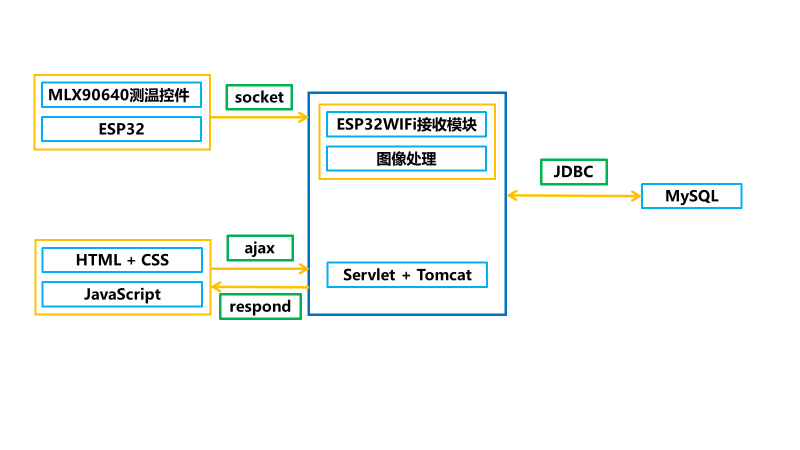
\includegraphics[width=0.8\textwidth]{design_1.png}
    \caption{总体设计}\label{fig:design_1}
    \vspace{\baselineskip}
    \end{figure}


\section{硬件系统设计}
硬件系统由MLX90640传感器和ESP32组成,开发环境为arduino。

主要分为两个部分来实现,首先是对传感器的数据进行采集。这一部分通过在网上收集资料,按照说明引入$MLX90640\_API.cpp$,$MLX90640\_I2C_Driver.cpp$中的函数来实现。

\begin{lstlisting} 
// 读取全部校正参数
    
int MLX90640_DumpEE(uint8_t slaveAddr, uint16_t *eeData) 
    
//解析校正参数为计算参数
    
int MLX90640_ExtractParameters(uint16_t * eeData,paramsMLX90640 *mlx90640) 
    
//读取一帧计算用实时数据
    
int MLX90640_GetFrameData(uint8_t slaveAddr, uint16_t *frameData) 
    
//得到外壳温度
    
float MLX90640_GetTa(uint16_t *frameData, const paramsMLX90640 *params)
    
//返回VDD电压值
   
float MLX90640_GetVdd(uint16_t *frameData, const paramsMLX90640 *params)
    
//返回绝对温度
   
void MLX90640_CalculateTo(uint16_t *frameData, const paramsMLX90640 *params, float emissivity, float tr, float *result)
    
    
\end{lstlisting}

另一部分的内容就是使用WiFi将获取到的数据发送出去。这里用到了ESP32的WiFi库,使用WiFi.begin()方法,传入WiFi名称和密码就可以连接。

对于需要更换网络环境这一问题,改进了WiFi的连接。启动时首先尝试连接上一次连接的WiFi,在一定时间内如果没有连接成功,则转为热点模式,此时可以通过手机连接热点,访问ESP32开设的小服务器,输入WiFi名称和密码,使其能够连接上新的WiFi。

发送数据用到的是WiFiClient,将得到的浮点数数组*100转为整形,拼接为字符串后后调用WiFiClient.print()方法即可将其发送出去。
\section{后端服务器设计}
后端服务器主要由两部分构成。第一部分是利用Java的socket通信接收ESP32通过WiFi发送的数据,将其读入float数组以待后续使用。
$Insertdata$类实现了二元和三元插值算法,将32*24像素的图像扩大至512*384像素并且满足图像及其轮廓符合人眼的生理观感。$PixelConversion$类实现了温度和可视颜色的伪彩编码转换,其中我们调整了温度在色条上的分布,使得其更加满足人体测温的需要,并且使得图像更加美观$Draw$类实现了图像的绘制。
将图像转换为Base64编码,使其能够在Web上显示。

另一部分利用了Servlet来实现,Servlet可以实现处理前端发送的http请求,生成动态的Web页面,从而能够将生成的图片的Base64编码持续发送给前端接收,实现热成像图片的实时显示。
\section{前端页面设计}
\section{数据库设计}
\begin{table}[htbp]
    \caption{admin表}\label{tab:table1}
    \vspace{0.5em}\centering\wuhao
    \begin{tabular}{ccccccc}
    \toprule[1.5pt]
    变量 & $id$ & $name$ & $account$&$password$ &$tel$&$email$\\
    \midrule[1pt]
    类型& int & varchar & varchar&varchar&varchar&varchar\\
    \bottomrule[1.5pt]
    \end{tabular}
    \vspace{\baselineskip}
    \end{table}
    
    \begin{table}[htbp]
        \caption{peoplelist表}\label{tab:table2}
        \vspace{0.5em}\centering\wuhao
        \begin{tabular}{cccccccc}
        \toprule[1.5pt]
        变量 & $id$&$address$ & $name$ & $tel$&$id_num$ &$tem$&$date$\\
        \midrule[1pt]
        类型& int & varchar & varchar&varchar&varchar&varchar&date\\
        \bottomrule[1.5pt]
        \end{tabular}
        \vspace{\baselineskip}
        \end{table}